\chapter{Implementation of Monitoring and Auto-Ballooning}
\label{chap:impl}

For the purpose of this thesis, we describe the implementation and experimentally evaluate only the monitoring and autoballooning parts of the DRS. The following sections describe the implementation details of these two components.

\section{Monitoring}
As we discussed in Chapter \ref{chap:design}, the monitoring component runs on each host and monitors the host and the guests running on that host to detect hotspots. The next few sections discuss which metrics are monitored, why they are monitored, and how they are monitored. Our implementation is done in the \textit{Python programming language}. The monitoring service runs periodically in every fixed time interval which is configurable. The default interval is set to then seconds. We will refer to this time interval as the \textit{monitor interval} in the rest of this document.

\subsection{Host Monitoring}
Monitoring the host is simple because the Linux kernel exposes much of the needed information stored in its internal data structure through procfs \cite{procfs}. Procfs is a filesystem in the Linux kernel, and hence can be accessed using the standard filesystem syscalls or through higher level API's that exist in almost all programming languages for this purpose. Since the DRS is running on the host, it has unhindered access to all the information in procfs.

\subsubsection{CPU Monitoring} \label{sec:cpumon}
For monitoring the CPU usage, we use the information in the  \textit{/proc/stat} file. The \textit{/proc/stat} file has the following fields capturing how much time CPU spent doing what task \cite{procfs}.

\begin{itemize}
\item \textbf{user:} time spent in executing normal processes in the user mode
\item \textbf{nice:} time spent in executing processes with positive nice value in the user mode
\item \textbf{system:} time spent in executing processes in kernel mode
\item \textbf{idle:} time for which the cpu was idle
\item \textbf{iowait:} time spent in waiting for I/O to complete
\item \textbf{irq:} time spent in servicing interrupts
\item \textbf{softirq:} time spent in servicing software interrupts
\item \textbf{steal:} time spent waiting involuntarily. This metric is relevant when the kernel running under virtualization, and its vCPU thread has to wait in the ready queue because the host CPU is overloaded.
\item \textbf{guest:} time spent running a normal guest (VM)
\item \textbf{guest\_nice:} time spent running a guest (VM) with positive nice value.
\end{itemize}
The time is measured in kernel jiffies. Jiffy is a counter that ticks on every timer interrupt. The interrupt frequency is 100Hz in majority of the systems.
From the above values, we can get the total time that has passed, and time for which the cpu was busy.
\begin{multline*}
 Total Time = user + nice + system + idle + iowait \\ + irq + iowait + irq + softirq + steal + guest + guest\_nice
\end{multline*}
$$ Busy Time = user + nice + system + irq + softirq + guest + guest\_nice$$

The $Total Time$ calculated here is the total time since the start of the system. Hence this will give the average cpu usage since the start of the system, which is not a useful metric for us. The average cpu usage in the previous monitor interval is more useful. To calculate that, we keep the $Total Time$ and $Busy Time$ at the previous monitor interval and subtract those values from the current values. So, 
$$
PrecentageCpuUsage = \frac{Busy Time - Previous Busy Time}{Total Time - Previous Total Time}*100$$

\subsubsection{Memory Monitoring} \label{impl:hostmemmon}
Memory usage information is present in the \textit{/proc/meminfo} file \cite{procfs}. For monitoring, we need several memory metrics which are described below.
\begin{itemize}
\item \textbf{Total memory:} The total usable memory present on the host. Present in the first line of the \textit{/proc/meminfo}.
\item \textbf{Used memory:} Total memory used by the host. This includes the memory used by the VMs, host's own processes and the page caches. This can be calculated by subtracting free memory, which is present in the second line of \textit{/proc/meminfo} file, from total memory.
\item \textbf{Available memory:} This provides an estimate of how much memory is available to any new application that will be started on the system. This is different from free memory because used memory also contains page caches, which can be reclaimed in case no free memory is left and an application requires more memory. Some of the slab memory used by the kernel is also reclaimable. The estimate also accounts for the fact that the system needs some page cache to function well, and that not all reclaimable slab can be reclaimed. It is present in the third line of \textit{/proc/meminfo} file.

Available memory is an important metric for us, because it basically tells us how much memory is available for the new VMs. It is better than free memory, because free memory does not take into account page caches which can be reclaimed.

\item \textbf{Hypervisor Load:} This is an important metric because we want to have a lower bound on how much memory is available for the hypervisor to function. We call this memory \textit{hypervisor reserved memory}. While calculating the amount of memory that is free for VMs to use, we do not want to use the memory that is reserved for the hypervisor.

For calculating the hypervisor load, we first calculate the VM load i.e.\ the amount of memory used by the virtual machines on the system. The VM load is calculated by looking at the RSS (resident set size) of all the virtual machines running on the host. Since QEMU-KVM treats each VM as a separate process, we need to get the RSS of all the processes which are running a virtual machine. The \textit{/proc/[pid]/statm} file has this information for each process. After calculating the VMlLoad, the hypervisor load is calculated as
$$Hypervisor Load = max(Hypervisor Reserved, Used Memory - Page Caches - VMLoad)$$

\item \textbf{Load Memory: } This metric represents the total memory that is loaded and hence, not available for use by any new VM or for existing VMs. It is calculated as
$$ 
Hypervisor Extra = max(Hypervisor Reserved-Hypervisor Load, 0)$$
$$Load Memory = (Total Memory - Available Memory - Idle Memory) + Hypervisor Extra$$

\item \textbf{Idle Memory: } Idle Memory is the memory which has been consumed by the VMs but is sitting idle inside the VM and can be ballooned out. Thus, it can be used by the existing VMs or any new VM that is migrated to the host. Its calculation is described later in the Section \ref{sec:guestmon}.
\end{itemize}

\subsection{Guest Monitoring} \label{sec:guestmon}
Monitoring a VM is more complex than monitoring the host because some of the metrics needed are not exposed by the VM to the host in any conventional way. Host operating system just gets to see the process abstraction of each virtual machine. So, the host has only as much information about each guest as it has about the rest of the processes running on it. In the next two sections, along with which metrics have been monitored, we have discuss some new techniques which we use to get some of the information from the guest VMs.

\subsubsection{CPU Monitoring}
CPU monitoring for a guest VM is straightforward because the host OS has the scheduling information for each process it is running. This information is exposed by the procfs. The metrics related to CPU utilization measured are discussed below.
\begin{itemize}
\item \textbf{Busy Time:} This is the time for which any of the vCPUs of the VM was scheduled onto any of the physical CPUs of the host. The scheduling information for each thread of a process is present inside the \textit{/proc/[pid]/task/[tid]/schedstat} file \cite{procfs}. We can get the busy time for each thread in nanoseconds from here. Adding the busy time for all the vCPU threads gives us the total busy time. The total time elasped has already been calculated in Section \ref{sec:cpumon}. We do calculation similar to Section \ref{sec:cpumon} to get the busy time percentage in previous monitor interval for all the guests.
\item \textbf{Steal Time:} Steal time \cite{ehrhardt2013cpu} is the time for which a vCPU thread waits in the ready queue while the CPU is busy executing some other process. Steal time has direct correlation to the amount of load on CPU and is useful in predicting whether the CPU is overloaded. Steal times for each thread is present inside the \textit{/proc/[pid]/task/[tid]/schedstat} \cite{procfs}. For each VM, we add the steal times of all its vCPU threads and calculate the average steal time percentage in the previous monitor interval.
\item \textbf{Estimated CPU Demand:} Estimated CPU demand is useful for predicting the amount of CPU a VM can consume if the host is not overloaded i.e.\ the steal time is 0. This value will be helpful during migration to check whether the CPU demands of the VM can be satisfied by the destination. It is calculated by adding a scaled value of steal percentage to the current busy percentage.
$$Estimated CPU DemandPrecent = \frac{Busy Time}{Total Time}*(1+\frac{Steal Time}{Total Time})*100 $$
\end{itemize}
\subsubsection{Memory Monitoring}
Getting the memory usage statistics is difficult because the host has no information about the memory management of the guest. The host only knows the amount of memory allocated by each guest. For calculating the idle memory of each guest, we need the amount of \textit{available memory} inside the VM.

One way for a guest VM to expose some information to the host is through a device driver. In a virtualized environment, all the devices available to a VM are virtual devices which are emulated by the hypervisor. So, a device driver running inside the VM can send some information to the device which is emulated by the hypervisor. The virtio balloon driver in the Linux kernel has a way of exposing the memory statistics to the host. It gives the total memory, free memory, swap in, major page faults, minor page fault metrics. We have modified the balloon driver to expose the available memory metric to the host too. We have also modified the backend virtio balloon hardware in QEMU to take the Available Memory metric from the balloon driver inside the guest. 
The following metrics related to the memory usage of the VMs are monitored. Figure \ref{fig:mem1} shows the relative sizes of different memory metrics calculated.
\begin{figure}[h]
  \centering
  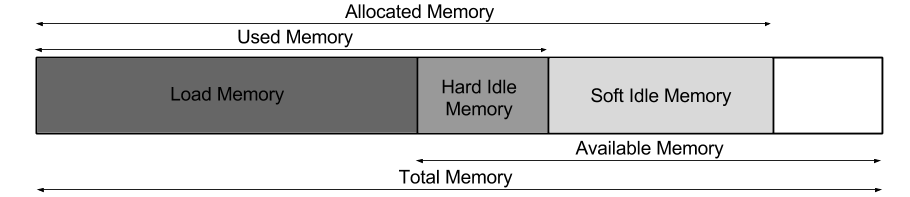
\includegraphics[width=\textwidth]{mem1.png}
  %\includegraphics{right-graph}
  \caption{Relative sizes of different types of memory metrics}\label{fig:mem1}
\end{figure}
\begin{itemize}
\item \textbf{Maximum Memory:} This is the maximum memory that the guest can have. The guest cannot be ballooned up after this point. We obtain this metric by using the API QEMU provides for this purpose.
\item \textbf{Current Memory:} This the amount of memory the guest has after taking the ballooned memory into account. From the point of view of the guest, this is its total memory, which can be increased or decreased by ballooning. The maximum limit for the current memory is the maximum memory. The \textit{total memory} statistic obtained through the virtio balloon driver represents this metric.
\item \textbf{Used Memory:} This is the memory which is being used by the guest. It includes all the page caches along with the memory being used by the processes inside the guest.
\item \textbf{Available Memory:} This is the amount of available memory inside the guest. The concept of available memory has been discussed in Section \ref{impl:hostmemmon}. We have modified the virtio balloon driver to obtain this metric.
\item \textbf{Allocated Memory:} This is the amount of memory of the guest that is backed by physical memory on the host. Allocated memory is different from current memory because the memory is allocated to the vritual machines on demand. This also may not equal to the used memory of the guest. Without ballooning, the memory, once allocated to a guest, is not reclaimed from it. So, the usage of a guest may keep on changing, but the allocated memory will always be equal to the maximum used memory in the guest's lifetime. Allocated memory is helpful in calculating the idle memory.

The allocated memory is calculated by looking at the virtual memory maps of the QEMU-KVM process corresponding to each VM. This information is present inside the \textit{/proc/[pid]/smaps} file \cite{procfs} for each process. The RAM of the guest VM is allocated by the QEMU process by doing a malloc of the size of maximum memory. Thus, it is one big contiguous chunk of memory in the heap memory of the process. From the information about different memory sections of the process present in this file, we look for the heap memory chunk of the size of VM's maximum memory. The RSS (resident set size) of this chunk of memory gives us the amount of memory in the VM that is backed by physical storage. 

In this chunk of allocated memory, there is some amount of memory that QEMU uses to store some metadata about the pages of the guest VM. Hence, this entire memory is not available to the guest. This part of memory cannot be reclaimed by ballooning. This overhead is constant and depends on the maximum memory size of the guest. We call this overhead as QEMU overhead. QEMU overhead needs to be deducted from the RSS. We use a piecewise continuous function to model the QEMU overhead. The values for the QEMU overhead in different scenarios were determined experimentally.
\[
QEMU Overhead =
  \begin{cases} 
      \hfill 200 MB    \hfill & \text{if $maxmem <= 4GB$} \\
      \hfill 300 MB \hfill & \text{if $ 4GB < maxmem <= 10GB$} \\
      \hfill 400MB \hfill & \text{if $ 10GB < maxmem <= 18GB$} \\
      \hfill 500MB \hfill & \text{if $ maxmem > 18GB$} \\
  \end{cases}
\]
$$ Allocated Memory = RSS - QEMU Overhead$$
\item \textbf{Load Memory:} This is the amount of memory that is loaded i.e.\ is being used by the processes of the guest and hence the current memory should not go below this point. 
$$Load Memory = Current Memory - Available Memory$$
\item \textbf{Idle Memory:} Idle memory is the amount of memory that is allocated, but is not being used by the guest, and hence, can be reclaimed. A lower bound on the current memory of the guest has been kept to avoid ballooning so much memory out of it that it is unable to function. This bound is called \textit{guest reserved}. So,
$$LowerBound = max(LoadMemory, GuestReserved)$$
$$Idle Memory = max(Allocated Memory - LowerBound, 0)$$
Based on how the idle memory is reclaimed, it can be divided into two types - hard idle memory and soft idle memory. Their importance and the difference between them have been explained in Section \ref{sec:bal}.
\end{itemize}

\subsection{Hotspot Detection and Key-Value Store Updation}
The hotspot detection algorithm should be robust enough not to generate false alarms. A simple threshold based algorithm which takes absolute or average values into account can raise many false alarms. Andreolini et al. \cite{andreolini2009dynamic} have shown the drawbacks of such algorithms and proposed a more robust statistical model to detect changes in the load profile of a machine which is based on the CUSUM (Cumulative Sum) algorithm \cite{page1957estimating}. We have used this algorithm for detecting hotspots and the time to update the key-value store. The algorithm is described below for the sake of completeness.

The hotspots due to memory overload are detected using the load memory metric of the host. The values for load memory are recorded in ever monitor interval to form a time series. Exponential average of the data is calculated as
$$ \mu_i = \alpha * loadmem_i + (1-\alpha)\mu_{i-1}$$
The value of $\alpha$ has been chosen to be $0.1$. The algorithm detects abrupt increase in  $\mu_i$ using $d_i$.
$$d_0 = 0;\ d_i = d_{i-1}+(loadmem_i - (\mu_i+K))$$
$d_i$ measures all the deviations from $\mu_i$ that are greater than $K$. $K=\frac{\Delta}{2}$ where $\Delta$ is the minimum shift to
be detected. It has been set to ($0.005*TotalMemory$) to detect minimum 1\% change in the value of $loadmem$. Change in the load profile of the host is triggered when $d_i > H$ where $H = h\sigma$, $h$ being a design parameter and $\sigma$ being the standard deviation of the time series upto that point. We have set $h=7$, which means that the load profile change is detected in an average of 14 samples \cite{andreolini2009dynamic}.
When the load-profile changes, the key-value store is updated with $totalmem - loadmem$. When the load profile changes and $(\mu_i > 0.8 * totalmem)$, hotspot is triggered and the migration service becomes active.

The hotspots in the CPU usage are also calculated in a similar way. The only difference is that the CUSUM algorithm runs on the steal time of all the guests, and any guest can trigger hotspot when its load profile changes and its $Average Steal Time > 10\%$. Additionally, the CUSUM algorithm runs on the busy time of the host to trigger the updation of the key-value store. The value stored in the key-value store is $(Number Of CPUs*100-BusyTimePercentage)$

\section{Auto-Ballooning}
Ballooning is a technique for increasing or decreasing the current memory of a guest. Auto-Ballooning is the process of automatically balancing memory amongst multiple guests running on a system by taking some memory from the idle guests and giving it to the needy guests. Auto-Ballooning is the most essential component for memory overcommitment.

\subsection{Hard Ballooning and Soft Ballooning} \label{sec:bal}
Depending upon the type of memory reclaimed ballooning can be classified into two types - hard ballooning and soft ballooning. Soft ballooning is the process of reclaiming memory which is free inside the guest while hard ballooning is the process of reclaiming memory which is used inside the guest.

\begin{align*}
&SoftLowerBound = max(Used Memory, Guest Reserved)\\
&Soft Idle Memory = max(Allocated Memory - SoftLowerBound, 0)\\
&Hard Lower Bound = max(Load Memory, Guest Reserved)\\
&Hard Idle Memory = max(Used Memory - Hard Lower Bound, 0)
\end{align*}

For soft ballooning, the guest is ballooned down to $(Current Memory - Soft Idle Memory)$, which will reclaim the SoftIdleMemory. To reclaim HardIdleMemory, the guest has to be ballooned down to $(Used Memory - Hard Idle Memory)$. Thus, ballooning down a guest from current memory to $(Current Memory - Soft Idle Memory)$ will reclaim SoftIdleMemory. After this, ballooning down from  $(Current Memory - Soft Idle Memory)$ to $Used Memory$ will reclaim no memory. Then, ballooning down from used memory to $(Used Memory - Hard Idle Memory)$ will reclaim the HardIdleMemory. Figure \ref{fig:mem2} shows the two different types of ballooning.

\begin{figure}[hb]
  \centering
  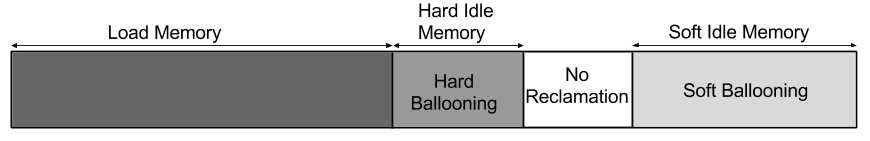
\includegraphics[width=\textwidth]{mem2.png}
  %\includegraphics{right-graph}
  \caption{Soft and hard ballooning}\label{fig:mem2}
\end{figure}

\subsection{Auto-Ballooning Algorithm}
The autoballooning algorithm first identifies the guests with idle memory and the guests which need more memory. We have already described the method of calculating the idle memory earlier. We identify needy guests as the ones whose average load memory is greater than a certain threshold. We have kept the threshold to $90\%$ of the current memory of the guest. Needy guests are ballooned up in intervals of $10\%$ of their current memory. Total needed memory is the sum total of the memory needed by all the needy guests(which is 10\% of the current memory for each needy guest).
\[
isNeedy(guest) =
  \begin{cases}
  	  \hfill True \hfill &  \text{$LoadMemory \ge 0.9*CurrentMemory$}\\
      \hfill False \hfill & \text{otherwise} \\
  \end{cases}
\]
$$ NeededMemory = 0.1*CurrentMemory$$

The \textit{host unused memory} is the amount of memory on the host which is neither used by/allocated to any guest nor is being used by the host, and hence, can be given away to any host by ballooning it up. Ballooning up a guest reduces the host unused memory, while ballooning a guest down decreases it. It is calculated as follows.
\begin{align*} 
Host Unused Memory = Available &Memory - Hypervisor Extra\\
&or\\
Host Unused Memory = Total Memory& - Load Memory - Total Idle Memory
\end{align*}
Auto-Ballooning can be triggered in two cases -  $(Host Unused Memory < 0.1*Total Memory)$ or $(Total Needed Memory>0)$.  The first case is important to keep the amount of swapped memory on the host low. To handle the first case, first the soft idle memory and then the hard idle memory form the guests is ballooned out till the $(Host Unused Memory < 0.2*Total Memory)$. If the idle memory is exhausted before this 20\% memory becomes unused, swapping is inevitable and the job of resolving it is left to the migration service.

%TODO: A figure here explaining ballooning algo in all the cases.
In the second case, either there is a needy guest or memory needs to be reclaimed for a guest which would be migrated to the machine. Both the situations are similar except that when memory is reclaimed for an incoming guest, there is no needy guest to be ballooned up. Depending on the needed memory and idle memory, three situations can arise.
\begin{enumerate}
\item $\mathbf{Total Needed Memory \le Total SoftIdleMemory.}$ The requirements of each needy guest can be satisfied by just soft-ballooning. So, the idle guests are ballooned down to reclaim the needed memory and then, the needy guests are ballooned up.
\item $\mathbf{TotalSoftIdleMemory < Total Needed Memory \le Total HardIdleMemory.}$ First, all the soft idle memory is ballooned out. Then, the rest of the needed memory is divided among the guests with hard idle memory in proportion of their hard idle memory. So, memory reclaimed by hard ballooning for a guest is given by
$$ NeedAfterSoftBallooning = TotalNeededMemory - TotalSoftIdleMemory$$
$$ Hard Reclaim = \frac{GuestHardIdleMem*NeedAfterSoftBallooning}{TotalHardIdleMemory}$$
Here, $GuestHardIdleMem$ is the hard idle memory for that particular guest, while $TotalHardIdleMem$ is the total hard idle memory. The reason hard ballooning is treated differently from soft ballooning is because soft ballooning is not supposed to have any affect on the performance of the guest as it takes away only the free pages. On the other hand, hard ballooning also reclaims some of the page caches, which might have some effect on the performance of the guest.
\item $\mathbf{Total Needed Memory > TotalHardIdleMemory.}$ This case implies that there is a hotspot on the host. Since the demands of all the guests cannot be satisfied, the memory is given to them or reclaimed from them based on their entitlement. The \textit{entitled memory} of each guest is calculated as
$$ EntitledMemory = GuestMaximumMemory*MemoryOvercommitmentRatio$$
After this, the idle memory and needed memory calculation is done again. 
$$ Idle Memory = max(Current Memory - Entitled Memory, 0)$$
\[
Needed Memory =
  \begin{cases}
  	  0 \ \ \ \ \ \ \ \ \ \ \ \ \   \text{if $!isNeedy(guest)$}\\
      0 \ \ \ \ \ \ \ \ \ \ \ \ \  Current Memory > Entitled Memory\\
      min(0.1*CurrentMemory,\\ \ \ CurrentMemory - Entitled Memory) \ \ \  \text{otherwise} \\
  \end{cases}
\]
Then, the idle memory is ballooned out of the guests and the needed memory is provided to the needy guests.

\subsection*{Summary}
In this chapter, we looked at the different techniques we use to monitor various metrics for hosts and guests. These metrics are used to trigger hotspot and make the ballooning service active. We also looked at the CUSUM based algorithm used to filter out unecessary spikes in the resource usage profiles of the host. In the end, we also discussed our technique of autoballooning.
\end{enumerate}

